% asset_id: OffSpecNumericalMethodsTikZ-001
% source: AI-proposed printable reconstruction of Euler diagram from supplied evidence
% status: Off-spec enrichment, not CCEA Further Mathematics core
\documentclass[tikz,border=8pt]{standalone}
\usepackage{amsmath}
\usetikzlibrary{arrows.meta,calc}
\definecolor{Canvas}{HTML}{FAF9F6}\definecolor{Ivory}{HTML}{FFFFF0}\definecolor{LineGrey}{HTML}{E5E5EA}\definecolor{AccentGold}{HTML}{C5A059}\definecolor{SoftPink}{HTML}{FBEFEF}\definecolor{TextMath}{HTML}{2C2C2E}\definecolor{Predicted}{HTML}{D94F70}\definecolor{Actual}{HTML}{7FB069}\definecolor{StartBlue}{HTML}{3D5A80}
\begin{document}
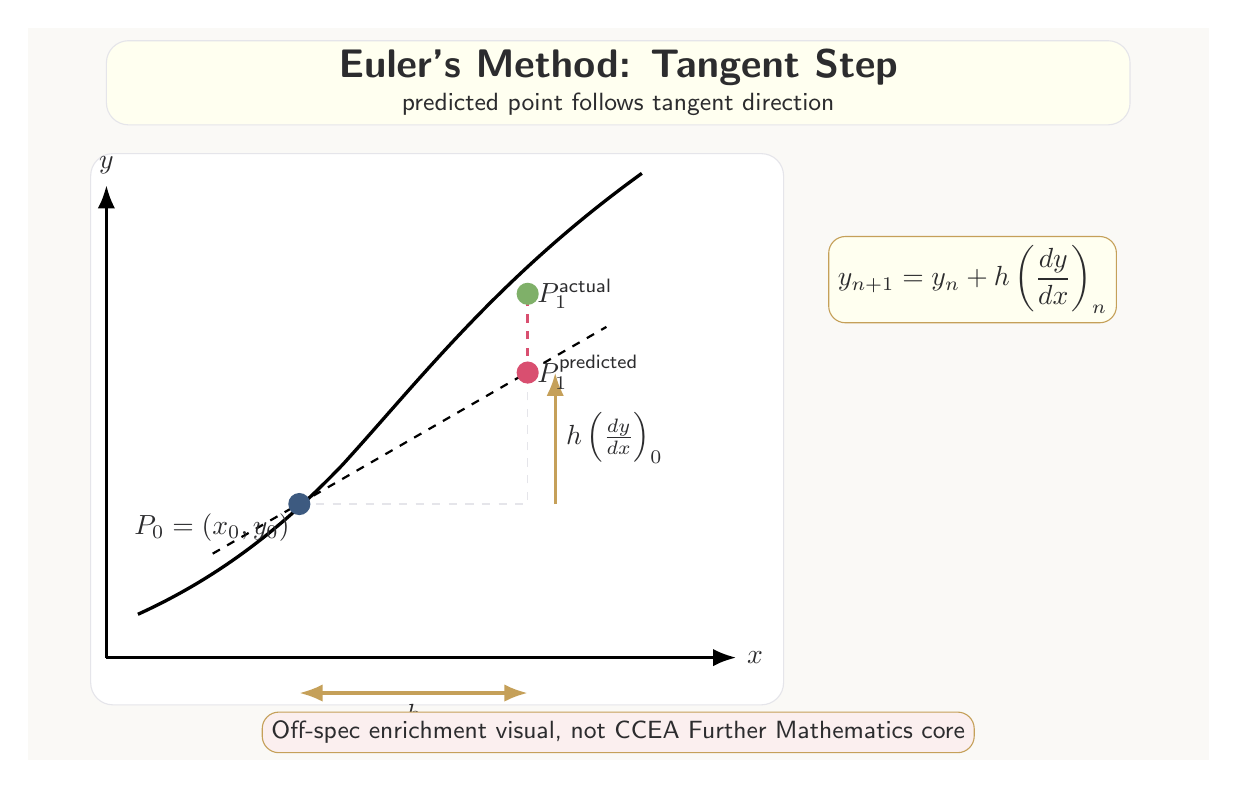
\begin{tikzpicture}[>=Latex,every node/.style={font=\sffamily,text=TextMath}]
\fill[Canvas] (-1,-1.3) rectangle (14,8);
\node[draw=LineGrey,fill=Ivory,rounded corners=8pt,minimum width=13cm,minimum height=1cm,align=center] at (6.5,7.3){\Large\textbf{Euler's Method: Tangent Step}\\\small predicted point follows tangent direction};
\draw[draw=LineGrey,fill=white,rounded corners=8pt] (-.2,-.6) rectangle (8.6,6.4);
\draw[->,very thick] (0,0)--(8,0) node[right]{$x$};\draw[->,very thick] (0,0)--(0,6) node[above]{$y$};
\draw[very thick] (.4,.55)..controls (1.5,1.05) and (2.3,1.72)..(3,2.45)..controls (4,3.55) and (5,4.85)..(6.8,6.15);
\coordinate(P0)at(2.45,1.95);\coordinate(Pp)at(5.35,3.62);\coordinate(Pa)at(5.35,4.62);
\draw[dashed,thick](1.35,1.32)--(6.35,4.20);\draw[dashed,LineGrey](P0)--(5.35,1.95)--(Pp);\draw[dashed,very thick,Predicted](Pp)--(Pa);
\draw[<->,very thick,AccentGold](2.45,-.45)--(5.35,-.45) node[midway,below]{$h$};\draw[->,very thick,AccentGold](5.7,1.95)--(5.7,3.62) node[midway,right]{$h\left(\frac{dy}{dx}\right)_0$};
\fill[StartBlue](P0)circle(4pt);\fill[Predicted](Pp)circle(4pt);\fill[Actual](Pa)circle(4pt);
\node[below left]at(P0){$P_0=(x_0,y_0)$};\node[right]at(Pp){$P_1^{\text{predicted}}$};\node[right]at(Pa){$P_1^{\text{actual}}$};
\node[draw=AccentGold,fill=Ivory,rounded corners=6pt,align=center] at (11,4.8){$\displaystyle y_{n+1}=y_n+h\left(\frac{dy}{dx}\right)_n$};
\node[draw=AccentGold,fill=SoftPink,rounded corners=6pt,align=center] at (6.5,-.95){\small Off-spec enrichment visual, not CCEA Further Mathematics core};
\end{tikzpicture}\end{document}
